\customHeader{1}{Splitting the Dataset}
\label{06_splitting_the_dataset}

As mentioned at the end of \headerName{} \ref{vsi_results_of_preprocessing}, after preprocessing, we obtain eight datasets for Binary \textclassification{}. For each dataset, we produce seven splits, two for training using \finetuning{} and five for training using \gls{pet}.


The most straightforward splitting method is for \finetuning{} on an unbalanced dataset. For each \contentType{}, such as the \translationTitle{}, we randomly split the dataset into 80\%-10\%-10\% for training, development, and testing, maintaining the original dataset's category distribution.

For \finetuning{} on a balanced dataset, we retain the split sizes and replicate the test split from the previous step. 
We then create balanced development and training segments by oversampling the positive category and randomly discarding from the negative category. Considering the original distribution was 90\% negatives to 10\% positives, we believe there will still be a sufficient representation of the negative category.

For \gls{pet}, we select a specific number of documents per category, for instance, 50. We then replicate the test and development splits from the balanced \finetuning{} split. From the balanced \finetuning{} training split, we select the first 50 documents from both the positive and negative categories to form the \gls{pet} training split (keeping in mind that \gls{pet} was first proposed for Few-shot learning). The remaining documents are used to construct the unlabeled split, by discarding their labels. Ditto for 100, 200, 500, and 1000 documents per category.

A detailed breakdown of the split sizes can be found in Appendix \ref{appendix04:statistics_for_splits}.


\putInBox{
This approach guarantees that for every \contentType{}, the test split remains consistent across all training methods. Maintaining the same test split for different training techniques ensures the \textbf{comparability} of our results. 
This is crucial, as performance on the test split assesses the classifier's effectiveness in real-world situations.
}

\begin{figure}
    \centering
    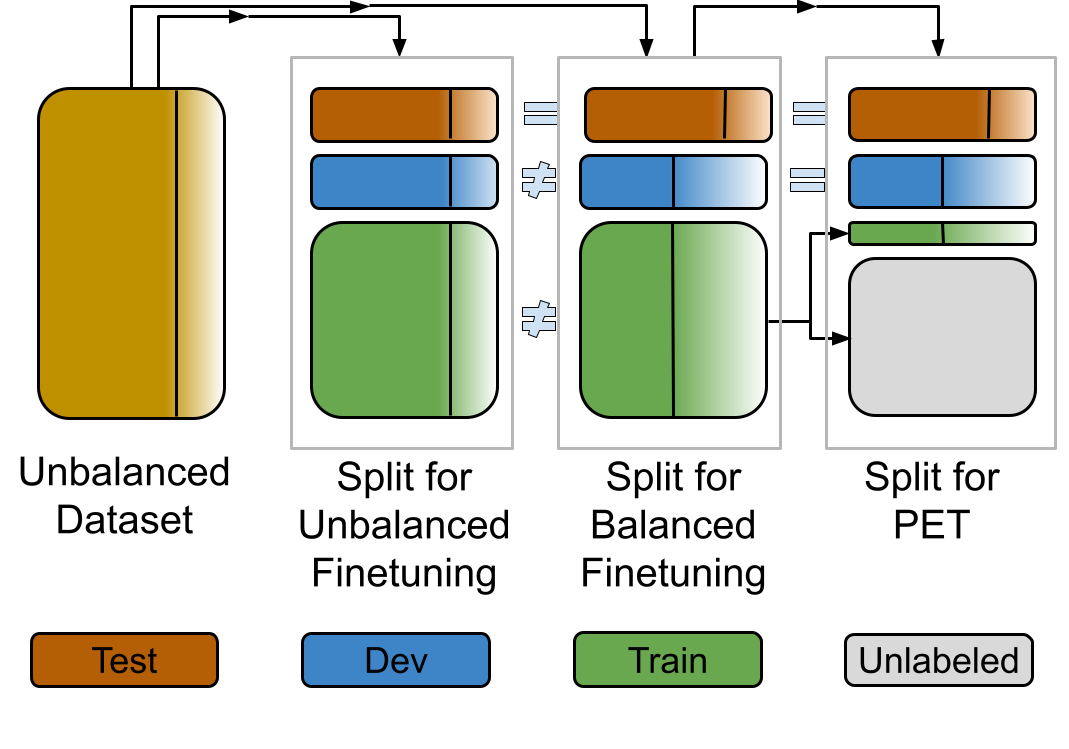
\includegraphics[width=0.5\textwidth]{Figures/06/06_dataset_splits.png}
    \caption{Strategies for Dataset Splitting}
    \label{fig:06_strategies_for_dataset_splitting}
\end{figure}